\chapter{Semi-Supervised Synset Similarity}
\label{chapter:Semi-SupervisedSynsetSimilarity}
In this chapter, we describe the idea of SimRank, its personalization and application to learning synset similarity in a semi-supervised fashion. Further we discuss how to coarsen the WordNet taxonomy and evaluate the clustering obtained in a WSD task based setting.

\section{Motivation}
The small coverage of the Support Vector Machines that we saw in section \ref{sec:supervisedAlgoOutline} makes them unsuitable to be used as a generic synset similarity estimator. To learn the similarity between synsets which do not share a word, we wish to utilize the relations encoded in WordNet as well as the information learnt using supervision. 
The ability of the Personalized SimRank framework to propogate the seeded information using semantic links between concepts allows us to learn complete synset similarity estimates.

\section{SimRank}
\label{sec:SimRank}
\subsection{Introduction}
SimRank \citep{Jeh02simrank} is a graph based similarity measure applicable in any domain with object-to-object relationships, with intuition that ``\textbf{two objects are similar if they are referenced by similar objects}'' \citep{Jeh02simrank} \citep{LizorkinSimrank}. Since SimRank has a recursive intuition, the base cases play an important role here.

Before discussing the model, let us introduce some notation for convenience. For a graph $G(V,E)$, for each node $v \in V$, we define the following:
\begin{itemize}
\item $I(v)$ is a set consisting of in-neighbours of node $v$ i.e.
\begin{equation}
I(v) = \{w\in V | (w,v)\in E\}
\end{equation}
\item $O(v)$ is a set consisting of out-neighbours of node $v$ i.e.
\begin{equation}
O(v) = \{u\in V | (v,u)\in E\}
\end{equation}
\end{itemize}

Individual members of $O(v)$ and $I(v)$ are referred to as $O_i(v)$, $1\leq i \leq |O(v)|$ and $I_j(v)$, $1\leq j \leq |I(v)|$.

Let $s(\alpha,\beta)$ denote the similarity score between objects $\alpha$ and $\beta$. The SimRank equation is given by: 
\begin{equation} \label{eq:SimRankBasic}
s(\alpha,\beta) =
\left\{ \begin{array}{rl}
1 & \mbox{if } \alpha=\beta \\
0 &  \mbox{ if } I(\alpha)=\phi \mbox{ or } I(\beta)=\phi \\
\frac{C}{|I(\alpha)||I(\beta)|}\sum_{i=1}^{|I(\alpha)|}\sum_{j=1}^{|I(\beta)|} s(I_i(\alpha),I_j(\beta)) & \mbox{ otherwise } \\
\end{array}\right.
\end{equation}
Here $C$ is a constant in range $(0,1)$ and is called the decay factor.

\subsection{Solution and its Properties}
\label{section:SimRankSolutionsAndProperties}
The solution to the SimRank equation \ref{eq:SimRankBasic} for a graph $G(V,E)$ is reached by iteration to a fixed-point. For each iteration $k$, we keep ${|V|}^2$ entries $S_k(\ast,\ast)$, where $S_k(\alpha,\beta)$ is the estimate of similarity between $\alpha$ and $\beta$ on $k^{th}$ iteration.
We start with $S_0(\ast,\ast)$ which is $1$ for singleton nodes like $(x,x)$, $0$ otherwise.

We successively compute $S_{k+1}(\ast,\ast)$ based on $S_k(\ast,\ast)$:
\begin{equation} \label{eq:SimRankBasicRecursive}
S_{k+1}(\alpha,\beta) =
\left\{ \begin{array}{rl}
1 & \mbox{if } \alpha=\beta \\
0 &  \mbox{if } I(\alpha)=\phi \mbox{ or } I(\beta)=\phi \\
\frac{C}{|I(\alpha)||I(\beta)|}\sum_{i=1}^{|I(\alpha)|}\sum_{j=1}^{|I(\beta)|} S_k(I_i(\alpha),I_j(\beta)) & \mbox{otherwise } \\
\end{array}\right.
\end{equation}

Let us highlight some properties of SimRank covered in \citep{Jeh02simrank} and \citep{LizorkinSimrank}:
\begin{enumerate}
\item A solution $s(\ast,\ast)$ to SimRank equations always exist and is unique, and $s(\ast,\ast) \in [0,1]$
\item For each $k$, $S_k(\ast,\ast)$ is upper bounded by the SimRank function $s(\ast,\ast)$ i.e.
\begin{equation}
 S_k(\alpha,\beta) \leq s(\alpha,\beta)
\end{equation}
\item Iterative functions $S_k(\ast,\ast)$ converge to SimRank function $s(\ast,\ast)$ i.e. 
\begin{equation}
\displaystyle \lim_{k \rightarrow \infty}S_k(\alpha,\beta)=s(\alpha,\beta)
\end{equation}
\item The difference between the SimRank scores and iterative similarity scores decreases exponentially in the number of iterations and uniformly for every pair of nodes i.e. 
\begin{equation} \label{SimRankExponentialConvergence}
s(\alpha,\beta) - S_k(\alpha,\beta) \leq C^{k+1} \mbox{\ \ \ \ }\forall \alpha,\beta \in V;\mbox{  } k=0,1,2\ldots
\end{equation}
\end{enumerate}

\subsection{Random Surfer Pair Model}
\citep{Jeh02simrank} show that the SimRank similarity score $s(\alpha,\beta)$ measures how soon two random surfers are expected to meet at the same node if they start at nodes $\alpha$ and $\beta$ and randomly walk the graph backwards.

\begin{equation}
s(\alpha,\beta) = \sum_{t:(\alpha,\beta) \rightsquigarrow (x,x)} P[t]C^{l(t)}  \label{eq:emd} 
\end{equation}

More formally, $s(\alpha,\beta)$ is the \textit{expected f-meeting distance} traveling back edges, between the nodes $\alpha$ and $\beta$ with $f(z)=C^z$.

\section{Personalized Weighted SimRank}
\subsection{Weighted SimRank}
Many times while working with real data, we observe relationships of different types between objects, which are likely to have different weights associated with them. For learning similarity between objects having such underlying structure, we discuss a weighted version of the SimRank method proposed in \citep{Jeh02simrank} and discussed in section \ref{sec:SimRank}. For convenience, let us define $W_{I}(n)$ and $W_{O}(n)$, for a node $n$ as follows:
\begin{align}
W_{O}(n) &= \sum_{i=1}^{|O(n)|} w(n,O_i(n)) \\
W_{I}(n) &= \sum_{i=1}^{|I(n)|} w(I_i(n),n)
\end{align}

The recursive equation for weighted SimRank is as follows:
\begin{align}
s(\alpha,\beta) = \frac{C}{W_{I}(\alpha)W_{I}(\beta)} \sum_{i=1}^{|I(\alpha)|} \sum_{j=1}^{|I(\beta)|} w(I_i(\alpha),\alpha) \cdot w(I_j(\beta),\beta) \cdot s(I_i(\alpha),I_j(\beta)) \label{eq:SimRankWeighted}
\end{align}

\noindent
The relation \ref{eq:SimRankWeighted} is obtained by extending the Random Surfer Pairs Model of SimRank and is discussed in more detail in Appendix \ref{appendix:weightedSimRank}.

\subsection{Personalizing SimRank}
\label{subsection:PersonalizedSimRank}
In many scenarios, while working with objects, we don't have complete information about the objects and thus have similarities for only some pair of objects. These similarities may be independently learnt and may not directly conform with the underlying graph. In such situations, we would like to get a more complete and consistent similarity metric between objects but we would like to use the information given to us as well. For the same, we propose a personalized framework for SimRank, in which we bias the SimRank by changing the initialization.
If we know similarities of some pairs, we fix them in our set of equations and let the rest of the values be automatically learned by the system.

Lets call the map of node pairs to their similarity values as $InitStore$. All the singleton nodes like $(x,x)$ have value equal to 1. The system of equations is defined as follows: 

\begin{equation} \label{eq:PersonalizedWeightedSimRank}
{\footnotesize
s(\alpha,\beta) =
\left\{ \begin{array}{rl}
1 & \mbox{if } \alpha=\beta\\
InitStore[(\alpha,\beta)] & \mbox{if } (\alpha,\beta) \in InitStore\\
\frac{C}{W_{I}(\alpha)W_{I}(\beta)} \sum_{i=1}^{|I(\alpha)|} \sum_{j=1}^{|I(\beta)|} w(I_i(\alpha),\alpha) \cdot w(I_j(\beta),\beta) \cdot s(I_i(\alpha),I_j(\beta)) & \mbox{otherwise }
\end{array}\right.
}
\end{equation}
In the personalized framework, we have no constraints over the initialization as long as all values initialized are in range $[0,C]$. 

\subsection{Solution of Personalized SimRank}
\label{section:ComputingPersonalizedSimRank}
A solution to the equations \ref{eq:PersonalizedWeightedSimRank} for a graph $G(V,E)$ is computed on lines of the method to solve equation \ref{eq:SimRankBasic} (refer section \ref{section:SimRankSolutionsAndProperties}). The successive computation of $S_{k+1}(\ast,\ast)$ from $S_k(\ast,\ast)$ is calculated as follows:
\begin{equation} \label{eq:PersonalizedWeightedSimRankSolution}
{\footnotesize
S_{k+1}(\alpha,\beta) =
\left\{ \begin{array}{rl}
1 & \mbox{if } \alpha=\beta\\
InitStore[(\alpha,\beta)] & \mbox{if } (\alpha,\beta) \in InitStore\\
\frac{C}{W_{I}(\alpha)W_{I}(\beta)} \sum_{i=1}^{|I(\alpha)|} \sum_{j=1}^{|I(\beta)|} w(I_i(\alpha),\alpha) \cdot w(I_j(\beta),\beta) \cdot S_k(I_i(\alpha),I_j(\beta)) & \mbox{otherwise}
\end{array}\right.
}
\end{equation}

All the properties of solution to SimRank equation are applicable to Personalized SimRank solution as well (refer section \ref{section:SimRankSolutionsAndProperties}). We prove all these properties for Personalized SimRank in Appendix \ref{appendix:PersonalizedSimRankProperties}.

\section{Personalized SimRank for Learning Synset Similarity}
\label{section:PersonalizedSimRankForLearningSynsetSimilarity}

%treating WordNet synsets as concepts

\subsection{Algorithm Outline}
\label{section:semiSupervisedAlgoOutline}
The Personalized SimRank framework requires an underlying graph $G(V,E)$, where $V$ is the set of objects to be clustered and $E$ is the set of semantic links connecting these objects and an $InitStore$ which contains the similarity values over some pairs from $V\times V$ learnt or known beforehand. Note that the values in the $InitStore$ have an upper bound of $C$.

For learning synset similarity, $V$ is the set of synsets to be clustered and $E$ is the set of WordNet relations connecting these synsets. We use the \textit{Hypernymy}, \textit{Hyponymy}, \textit{Meronymy} and \textit{Holonymy} relations of WordNet as the semantic links. We seed the $InitStore$ as follows:
\begin{itemize}
\item We predict the similarity values of all the synset pairs which share at least one word using the Support Vector Machine learnt from synset-merging data from OntoNotes \citep{Hovy:2006} as described in section \ref{sec:ClassifierAndTraining}.
\item We transform the SVM predictions to the range $[0,1]$ using the sigmoid model learnt on the OntoNotes dataset. (see section \ref{sec:EstimatingPosteriorProbabilitiesFromSVMScores})
\item We scale the posterior probabilities obtained to range between $[0,C]$ by linear scaling, where $C$ is the SimRank decay parameter.
\end{itemize}

\subsection{Estimating Posterior Probabilities from SVM Scores}
\label{sec:EstimatingPosteriorProbabilitiesFromSVMScores}
Given a set of training examples $x_i \in \mathbb{R}^n, i=1,\ldots,t,$ labeled by $y_i \in \{-1,+1\}$ with $N_+$ positive examples and $N_-$ negative examples, a Support Vector Machine finds a maximum margin decision boundary $f(x)$ whose sign serves as a label prediction for any test example $x$. Instead of label prediction, many systems, as in our case: SimRank Initialization, require posterior probability $Pr(y= +1|x)$ estimate. 
\citep{Platt99} proposed approximating the posterior by a sigmoid function
\begin{align}
Pr(y=+1|x) \approx P_{A,B}(f(x)) \equiv \frac{1}{1+exp{(Af(x)+B)}}
\end{align}

To avoid overfitting of the sigmoid, an out-of-sample model is used i.e. for each training example target values $t_i$s are used (instead of 1 and 0), where 
\begin{equation} \label{eq:SVMTargetValues}
t_i =
\left\{ \begin{array}{rl}
\frac{N_+ +1}{N_+ +2} & \mbox{if } y_i = +1\\
\frac{1}{N_- +2} & \mbox{if } y_i = -1\\
\end{array}\right.
\end{equation}

Let each $f_i$ be shorthand for $f(x_i)$. 
The best parameter setting $z^{\ast} = (A^{\ast},B^{\ast})$ is determined by solving the following regularized maximum likelihood problem:
\begin{align} \label{eq:regularizedMLProblem}
\displaystyle \min_{z=(A,B)} F(z) = - \sum_{i=1}^{t}\left( t_i \log(P_{A,B}(f_i)) + (1-t_i)\log(1-P_{A,B}(f_i))\right)
\end{align}

\citep{Platt99} indicated that for solving equation \ref{eq:regularizedMLProblem}, any method for unconstrained optimization can be used. We use Newton's method with backtracking, as proposed in \citep{Lin03Note}, as it avoids numerical difficulties faced by \citep{Platt99}. The pseudocode for the implementation is available in Appendix \ref{appendix:SVMProb}.

\subsection{Importance of Parameter \texorpdfstring{$C$}{TEXT} }
The parameter $C$ in Personalized SimRank affects the algorithm in many ways:
\begin{itemize}
\item \textbf{Maximum Similarity between distinct objects}: According to the SimRank equations, the maximum similarity between two distinct objects can be at most $C$.

\begin{align}
s(a,b) &= \frac{C}{W_{I}(a)W_{I}(b)} \sum_{i=1}^{|I(a)|} \sum_{j=1}^{|I(b)|} w(I_i(a),a)  \cdot w(I_j(b),b) \cdot \underbrace{s(I_i(a),I_j(b))}_{\leq 1}\\
&\leq \frac{C}{W_{I}(a)W_{I}(b)} \sum_{i=1}^{|I(a)|} \sum_{j=1}^{|I(b)|} w(I_i(a),a)  \cdot w(I_j(b),b)\\
&\leq \frac{C}{W_{I}(a)W_{I}(b)} \left( \sum_{i=1}^{|I(a)|} w(I_i(a),a) \right )  \cdot \left( \sum_{j=1}^{|I(b)|}  w(I_j(b),b) \right )\\
&\leq C
\end{align}

\item \textbf{Rate of convergence}: The rate of convergence of the iterative method to find the solution for SimRank equations is dependent on $C$ as there is exponential decrease in the difference between SimRank theoretical and iterative similarity scores in the number of iterations. In short, the higher the value of $C$, the slower is the convergence.
\end{itemize}

To understand the importance of the parameter $C$, we vary the value of $C$ in our experiments and empirically study the results obtained.

\section{Coarsening WordNet}
In this section we would discuss our method to cluster synsets of WordNet, which would give us coarser senses for words. The task in hand can be described as follows: Assuming we have a similarity metric which gives us similarity between each pair of synsets, we need to cluster the synsets where the granularity of the clustering can be adjusted according to the needs of the application.

We use the similarity metric learnt using the personalized SimRank model as described in section \ref{section:PersonalizedSimRankForLearningSynsetSimilarity}.
We construct a graph $G(V,E)$ where the vertices $V$ are the synsets of the WordNet graph and edges $E$ are obtained by thresholding the similarity metric.
On this graph, we find connected components, which gives us a partition over synsets.
The algorithm \ref{alg:CoarseningWordNet} summarises our method:

\begin{algorithm}[h]
\begin{algorithmic}[1]
 \State \textbf{Input: } WordNet Graph $WN(V,E)$, Similarity Metric $Sim$ and threshold $t$
 \State \textbf{Output: } Partition over $V$ 
 \State $E' \gets \emptyset$
 \ForAll{Synset $s_i \in V$}
  \ForAll{Synset $s_j \in V$}
    \If{$Sim(s_i,s_j) \geq t$} 
    $E' \gets E' \cup (s_i,s_j)$
    \EndIf
  \EndFor
 \EndFor 
 \State $C \gets ConnectedComponents(G(V,E'))$\\
 \Return $C$
\end{algorithmic}
\caption{Coarsening WordNet}
\label{alg:CoarseningWordNet}
\end{algorithm}

We use the clustering obtained to derive coarse senses of words. For a word, all its senses in the same cluster are merged and act as a coarse sense. Algorithm \ref{alg:QueryingSenses} summarises the querying method:

\begin{algorithm}[h]
\begin{algorithmic}[1]
 \State \textbf{Input: } WordNet Graph $WN(V,E)$, Word $w$ and Partition $P$ over $V$ 
 \State \textbf{Output: } Set of coarse senses $C$
 \State $L \gets ListSenses_{WN}(w)$
 \State $C \gets \emptyset$
 \ForAll{Synset $s_i \in L$}
  \State $C \gets C \cup \{s_i\}$
 \EndFor 
 \ForAll{Synset $s_i \in L$}
  \ForAll{Synset $s_j \in L$}
    \If{$s_i \neq s_j$ and $P(s_i,s_j) == 1$} 
    $C \gets Merge(C,s_i,s_j)$
    \EndIf
  \EndFor
 \EndFor  \\
\Return $C$
\end{algorithmic}
\caption{Querying Senses of a word}
\label{alg:QueryingSenses}
\end{algorithm}

\section{Experimental Setup and Evaluation}
\label{section:evaluation}
\subsection{Estimating Posterior Probabilities from SVM Scores}
We learn the parameters $A$ and $B$ of the sigmoid transforming SVM predictions to posterior probabilities (see section \ref{sec:EstimatingPosteriorProbabilitiesFromSVMScores}). Using the same data set that was used to train the model we want to calibrate will introduce unwanted bias. So we used an independent calibration set in order to get good posterior probabilities \citep{Niculescu-Mizil:2005}.

We address this problem by calibrating on an independently generated random balanced subsets from OntoNotes (see section \ref{sec:OntoNotesDataset}). The SVM predictions are obtained using the SVMs trained over random subsets of the OntoNotes data (see section \ref{section:SupervisedExperimentalSetupAndEvaluation}). Since all the SVMs were trained on randomly generated datasets, we selected the SVM that performed the best in cross validation.

The values of $A$ and $B$ obtained are -1.1655 and 0.0222 respectively. Using these values, the SVM prediction of value 0 gets mapped to 0.4944. 

\subsection{Semi-Supervised Similarity Learning}
We learn similarity models using the SimRank variant described in section \ref{section:semiSupervisedAlgoOutline}. \citep{Jeh02simrank} use $C=0.8$ and report that 5-6 iterations are enough. \citep{LizorkinSimrank} suggest to use lower values of $C$ or more number of iterations. We vary the values taken by $C$ as 0.6, 0.7 and 0.8. We run all the systems for 10 iterations to avoid convergence issues. 

We use the \textit{Hypernymy}, \textit{Hyponymy}, \textit{Meronymy} and \textit{Holonymy} relations of WordNet as the semantic links. All the semantic links used in all the experiments have uniform weight unity. For implementation, we used EZGraph Java library\footnote{ezgraph - Easy to Use Graph Analysis Library:  \url{https://code.google.com/p/ezgraph/}}.

\subsection{Coarsening WordNet}
We assess the effect of automatic synset clustering on the English all-words task at Senseval-3 \citep{Senseval3AllWordsTask} (this evaluation is similar to the evaluation used by \citep{Navigli06meaningfulclustering} and \citep{snow07mergesense}). The task asked WSD systems to select the apt sense for 2,041 content words in running texts comprising of 351 sentences. Since we focus on nouns, we used the 890 instances labelled with noun as the part of speech.

We consider the three best performing WSD systems: GAMBL \citep{decadt-EtAl:2004:Senseval-3}, SenseLearner \citep{mihalcea-faruque:2004:Senseval-3} and Koc University \citep{yuret:2004:Senseval-3} - and the best unsupervised system: IRST-DDD \citep{strapparava-gliozzo-giuliano:2004:Senseval-3} submitted in the task. The answer by the system is given full credit if it belongs to the cluster of the correct answer.

Observe that any clustering will only improve the WSD performance. Therefore to assess the improvement obtained because of our particular clustering, we calculate the expected performance for a random clustering at the same granularity as our clustering and study the improvement over random clustering instead. 

Score for a random clustering is calculated as follows: Let the word to be disambiguated have $N$ senses, each mapped to a unique synset. Let the clustering of these $N$ synsets on a particular granularity give us $k$ clusters $C_1,\ldots C_k$. The expectation that an incorrectly chosen sense and the actual correct sense would be in cluster $C_i$  in this clustering is $\frac{|C_i|(|C_i|-1)}{N(N-1)}$. Using linearity of expectation, we can say that the chances of the two synsets belonging to same cluster would be 
\begin{equation}
\frac{\sum_{i=1}^{k} |C_i|(|C_i|-1) }{N(N-1)}
\end{equation}

We experiment with $C$ = 0.6, 0.7 and 0.8. The SVM probability boundaries when scaled to $[0,C]$ for these values are 0.30, 0.35 and 0.40. So for finding the threshold giving the best improvement against random clustering baseline, we use the search space $[C-0.35, C]$. The performance of the systems at these thresholds for different values of $C$ is reported in %tables \ref{tab:wsdImprovement0.6}, \ref{tab:wsdImprovement0.7} and \ref{tab:wsdImprovement0.8}.
table \ref{tab:wsdImprovement}.

% \begin{center}
% \begin{longtable}{| c || c | c | c | c | c |}      
%     \hline
%     System & F-Score & Threshold & CCC & Random & Improvement \\ \hline
%     GAMBL & 0.7116 & 0.36 & 0.9031 & 0.8424 & 0.0607 \\ \hline
%     SenseLearner & 0.7104 & 0.37 & 0.8824 & 0.8305 & 0.0518 \\ \hline
%     KOC University & 0.7191 & 0.37 & 0.8924 & 0.8314 & 0.0610 \\ \hline
%     IRST-DDD & 0.6367 & 0.35 & 0.8731 & 0.8013 & 0.0718 \\ \hline
%     \caption{Improvement in Senseval-3 WSD performance using Connected Component Clustering Vs Random Clustering at the same granularity with C = 0.6}
%   \label{tab:wsdImprovement0.6}
% \end{longtable}
% \end{center}
% 
% \begin{center}
% \begin{longtable}{| c || c | c | c | c | c |}      
%     \hline
%     System & F-Score & Threshold & CCC & Random & Improvement \\ \hline
%     GAMBL & 0.7116 & 0.52 & 0.8453 & 0.7864 & 0.0589 \\ \hline
%     SenseLearner & 0.7104 & 0.49 & 0.8541 & 0.8097 & 0.0444 \\ \hline
%     KOC University & 0.7191 & 0.52 & 0.8448 & 0.7911 & 0.0538 \\ \hline
%     IRST-DDD & 0.6367 & 0.49 & 0.7970 & 0.7402 & 0.0568 \\ \hline
%     \caption{Improvement in Senseval-3 WSD performance using Connected Component Clustering Vs Random Clustering at the same granularity with C = 0.7}
%   \label{tab:wsdImprovement0.7}
% \end{longtable}
% \end{center}
% 
% \begin{center}
% \begin{longtable}{| c || c | c | c | c | c |}      
%     \hline
%     System & F-Score & Threshold & CCC & Random & Improvement \\ \hline
%     GAMBL & 0.7116 & 0.59 & 0.8419 & 0.7843 & 0.0577 \\ \hline
%     SenseLearner & 0.7104 & 0.56 & 0.8439 & 0.7984 & 0.0455 \\ \hline
%     KOC University & 0.7191 & 0.59 & 0.8414 & 0.7879 & 0.0535 \\ \hline
%     IRST-DDD & 0.6367 & 0.47& 0.8881 & 0.8324 & 0.0557 \\ \hline
%     \caption{Improvement in Senseval-3 WSD performance using Connected Component Clustering Vs Random Clustering at the same granularity with C = 0.8}
%   \label{tab:wsdImprovement0.8}
% \end{longtable}
% \end{center}

%%%%%%%%%%%%%%%%%%%%%%%%%%%%

\begin{center}
\begin{longtable}{|c| c || c | c | c | c | c |}      
    \hline
    C & \textbf{System} & \textbf{F-Score} & \textbf{Threshold} & \textbf{CCC} & \textbf{Random} & \textbf{Improvement} \\ \hline
    \multirow{4}{*}{0.6} & GAMBL & 0.7116 & 0.36 & 0.9031 & 0.8424 & 0.0607 \\ \cline{2-7}
    & SenseLearner & 0.7104 & 0.37 & 0.8824 & 0.8305 & 0.0518 \\ \cline{2-7}
    & KOC University & 0.7191 & 0.37 & 0.8924 & 0.8314 & 0.0610 \\ \cline{2-7}
    & IRST-DDD & 0.6367 & 0.35 & 0.8731 & 0.8013 & 0.0718 \\ \cline{2-7}
    \hline    
    \multirow{4}{*}{0.7} & GAMBL & 0.7116 & 0.52 & 0.8453 & 0.7864 & 0.0589 \\ \cline{2-7}
    & SenseLearner & 0.7104 & 0.49 & 0.8541 & 0.8097 & 0.0444 \\ \cline{2-7}
    & KOC University & 0.7191 & 0.52 & 0.8448 & 0.7911 & 0.0538 \\ \cline{2-7}
    & IRST-DDD & 0.6367 & 0.49 & 0.7970 & 0.7402 & 0.0568 \\ \cline{2-7}
    \hline    
    \multirow{4}{*}{0.8} &GAMBL & 0.7116 & 0.59 & 0.8419 & 0.7843 & 0.0577 \\ \cline{2-7}
    & SenseLearner & 0.7104 & 0.56 & 0.8439 & 0.7984 & 0.0455 \\ \cline{2-7}
    & KOC University & 0.7191 & 0.59 & 0.8414 & 0.7879 & 0.0535 \\ \cline{2-7}
    & IRST-DDD & 0.6367 & 0.47& 0.8881 & 0.8324 & 0.0557 \\
    \hline
    \caption{Improvement in Senseval-3 WSD performance using Connected Component Clustering Vs Random Clustering at the same granularity}
  \label{tab:wsdImprovement}
\end{longtable}
\end{center}

Commenting theoretically about the impact of $C$ on the performance is tough as by changing $C$ we are changing all the ${|V|}^2$ simultaneous equations to be solved. Empirically we observe that improvements over baseline keep on decreasing on increasing $C$ across all the systems. It might be because of the slow convergence of SimRank for higher values of $C$.

We observe from the figures \ref{fig:supervisedSystemsImprovement} and \ref{fig:unsupervisedSystemsImprovement} that by varying thresholds, the improvement of the Connected Components Clustering over the random clustering baseline at the same granularity first increases and then decreases.

Across supervised and unsupervised systems, we observe that the unsupervised systems obtain higher improvements than the supervised systems which can be attributed to fact that the unsupervised system used was underperforming compared to the supervised systems in the fine grained WSD task setting.

\begin{figure}
\centering
\subfigure[]{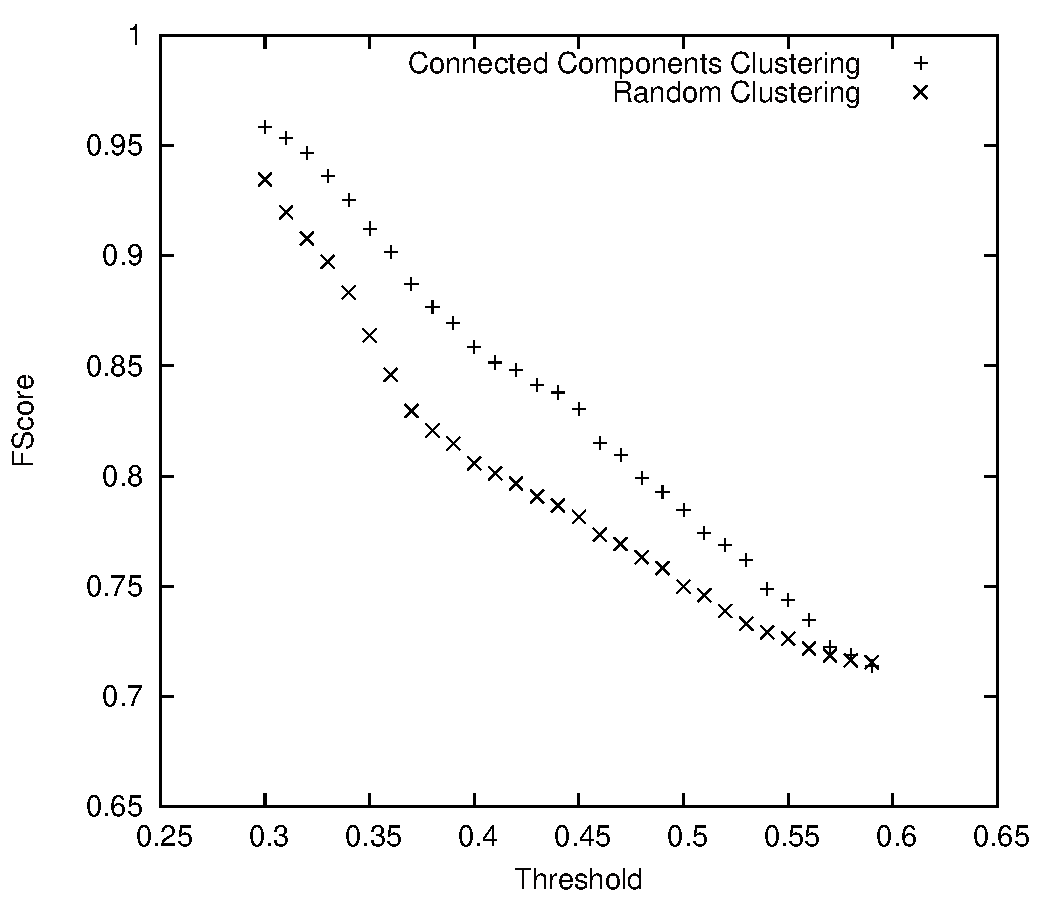
\includegraphics[width=2.9in]{SVMScaledSupervised6.pdf}\label{superviseda}}
\subfigure[]{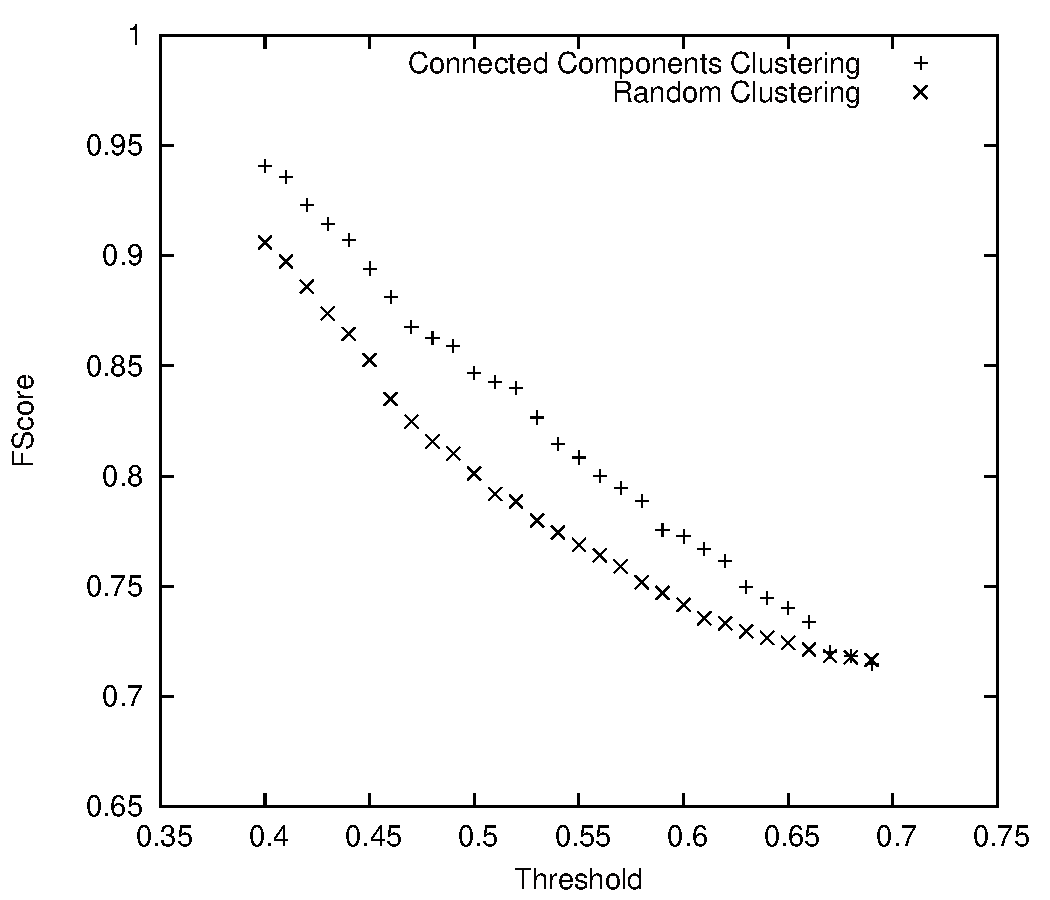
\includegraphics[width=2.9in]{SVMScaledSupervised7.pdf}\label{supervisedb}}
\subfigure[]{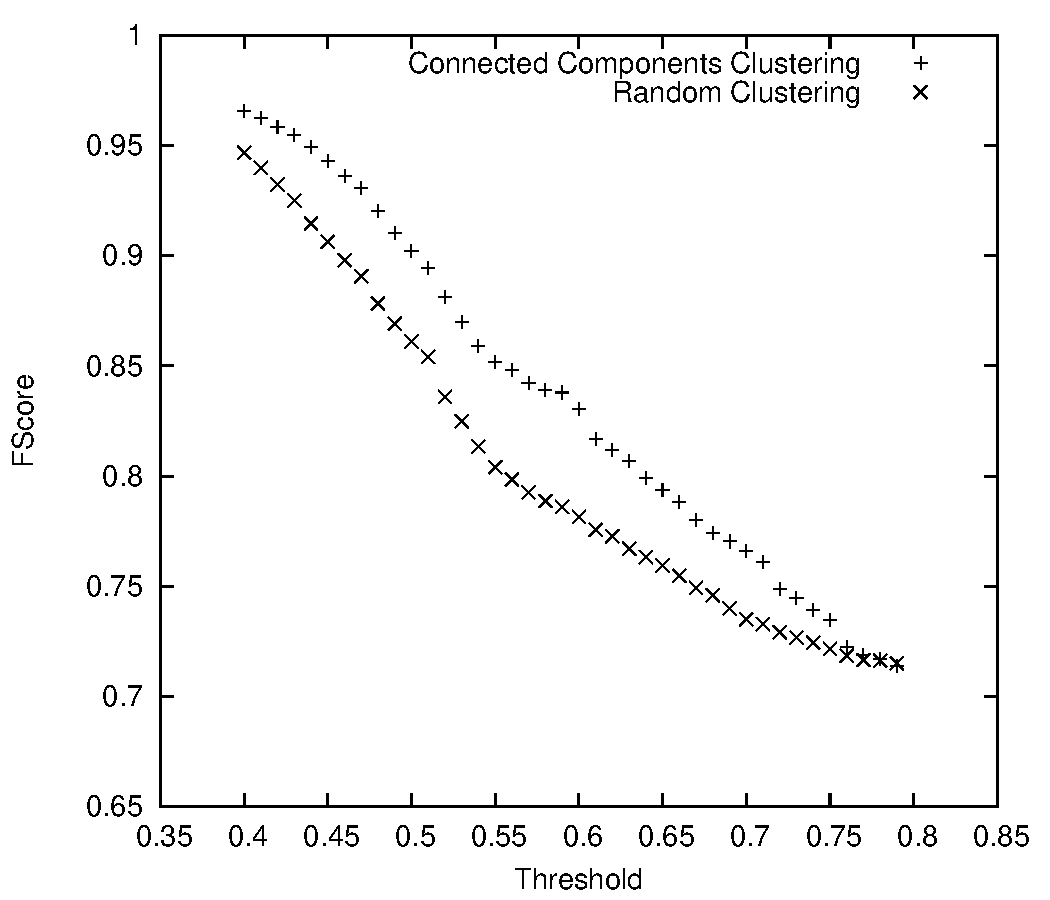
\includegraphics[width=2.9in]{SVMScaledSupervised8.pdf}\label{supervisedc}}
\caption{Improvement in average performance of best 3 Supervised Systems in Senseval-3 using Connected Component Clustering Vs Random Clustering at the same granularity with C = (a) 0.6, (b) 0.7 and (c) 0.8}
\label{fig:supervisedSystemsImprovement}
\end{figure}

\begin{figure}
\centering
\subfigure[]{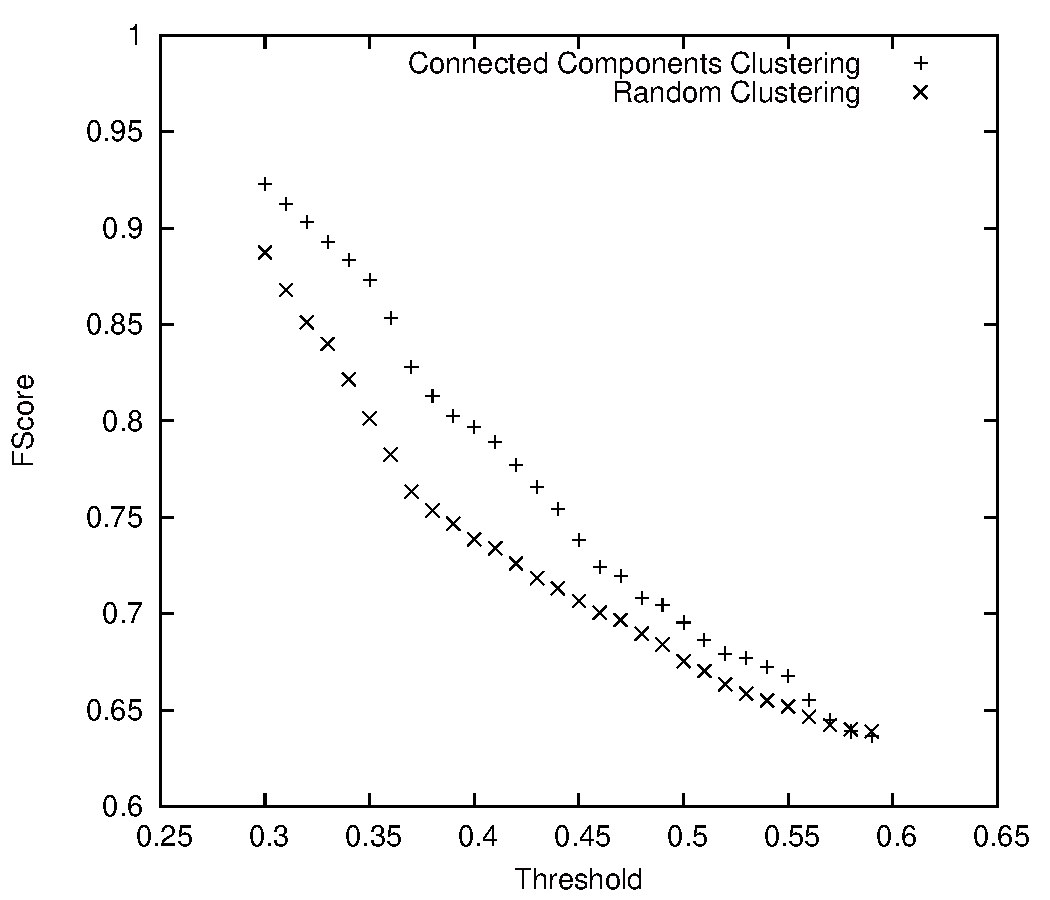
\includegraphics[width=2.9in]{SVMScaledUnsupervised6.pdf}\label{unsuperviseda}}
\subfigure[]{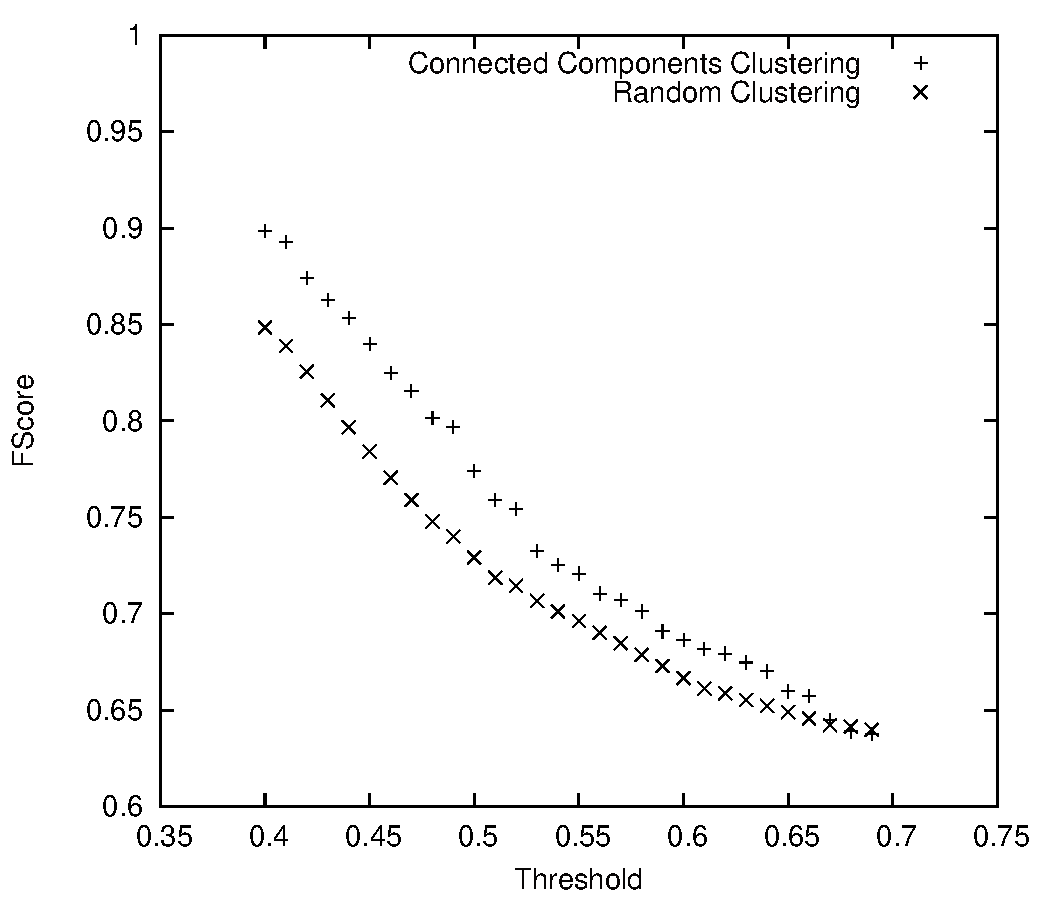
\includegraphics[width=2.9in]{SVMScaledUnsupervised7.pdf}\label{unsupervisedb}}
\subfigure[]{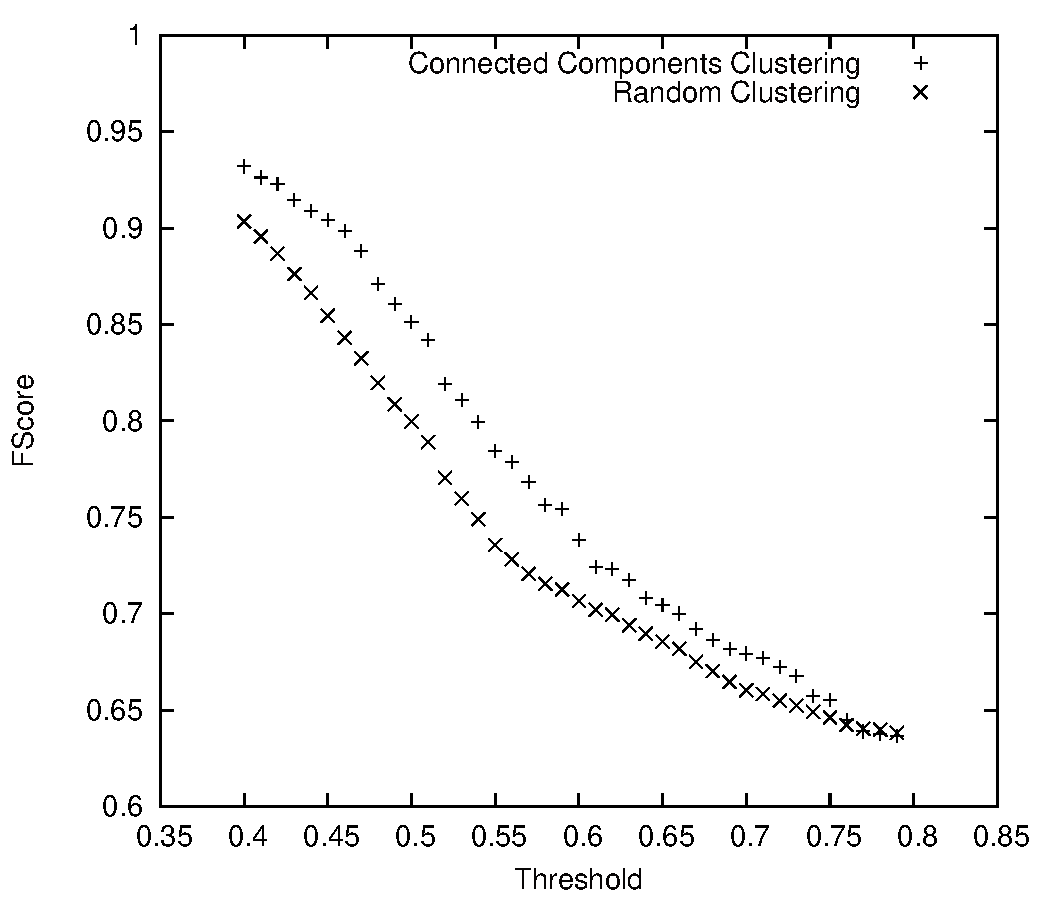
\includegraphics[width=2.9in]{SVMScaledUnsupervised8.pdf}\label{unsupervisedc}}
\caption{Improvement in performance of best Unupervised System in Senseval-3 using Connected Component Clustering Vs Random Clustering at the same granularity with C = (a) 0.6, (b) 0.7 and (c) 0.8}
\label{fig:unsupervisedSystemsImprovement}
\end{figure}

\section{Conclusions and Future Work}

\subsection{Conclusions}
The method discussed in the chapter learns a model for calculating synset similarity utilizing the taxonomy information and information learnt from manually obtained sense clustering. The framework obtained is generic and can be applied to other parts of speech as well.

For coarsening senses, we proposed one of the simplest approaches to cluster senses but it can be made to work with any clustering algorithm to generate coarse senses. We show that the clustering obtained by partitioning synsets in  connected components gives us a maximum improvement of 5.78\% on supervised systems and 7.18\% on unsupervised system.

\subsection{Future Work}

\subsubsection{Differentiating WordNet relations}
We use the WordNet relations \textit{Hypernymy}, \textit{Hyponymy}, \textit{Meronymy} and \textit{Holonymy} without any differentiation i.e. weights of all the links are unity. If we can grade the weights of the relations based on their relative importances, we can expect an improvement in the system. One way can be to perform cognitive experiments and obtain the weights of relations from the feedback of the annotators. An alternative way can be learn weights in a task based setting using an approach similar to \citep{Navigli05SSI}.

\subsubsection{Speeding up the implementation}
We used the naive implementation of SimRank, proposed in \citep{Jeh02simrank}, for implementing Personalized SimRank. Faster approximate scalable implementations of SimRank like \citep{FogarasSimRank}, \citep{LizorkinSimrank} etc. can also be adapted appropriately for personalization and thus speed up the algorithm.

